\documentclass[12pt,a4paper]{article}
\usepackage{rmpackages}																% usual packages
\usepackage{rmtemplate}																% graphic charter
\usepackage{rmexocptce}																% for DS with cptce eval

\cfoot{} 													% if no page number is needed
%\renewcommand\arraystretch{1.5}		% stretch table line height

\begin{document}

\begin{header}
Les défis confinés -- Épisode 6 
\end{header}

\section*{Réaliser une chronophotographie}

Une chronophotographie est une image réalisée à partir d'une succession de photographies prises à intervalles de temps réguliers.
Ci-dessous, on voit une chronophotographie réalisée à partir de quatre photos du même oiseau en plein vol.
Le photographe est au sol et son appareil photo est fixe.

\begin{center}
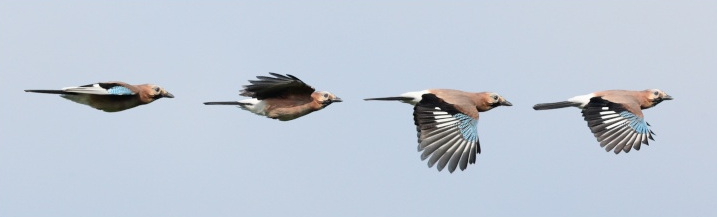
\includegraphics[width=\textwidth]{images/chrono_bird.png}
\end{center}

\begin{enumerate}
\item Décrire le mouvement (trajectoire et vitesse) de cet oiseau par rapport au sol.

\item Reproduire cette chronophotographie en modélisant l'oiseau par un point.

\item Avec l'application Cliché Mouvement (ou Motion Shot) disponible sur smartphone, réaliser la chronophotographie d'un système de votre choix et poster le résultat dans la conversation du groupe de physique-chimie sur Teams.

\item Sous votre photo, toujours dans Teams, proposer une légende en indiquant :
\begin{itemize}
\item[•] le système étudié ;
\item[•] le référentiel choisi pour l'étude ;
\item[•] la nature de la trajectoire ;
\item[•] si le mouvement est uniforme ou non.
\end{itemize}
\end{enumerate}

\section*{Pour info}

Le 18 février 2021, Perseverance se posait sur Mars.
Il s'agit d'un rover de la NASA qui va chercher des signes de vie passée sur Mars et préparer des échantillons de sol qui seront un jour ramenés sur Terre.

Si vous ne l'avez pas vue, le lien ci dessous vous mènera vers la vidéo de l'atterrissage : \href{https://youtu.be/4czjS9h4Fpg}{https://youtu.be/4czjS9h4Fpg}.
Les sous-titres français sont disponible via la traduction automatique de sous-titres.

\end{document}